\section{Криптосистемы-протоколы}\label{section-cryptosystems-protocols}
\selectlanguage{russian}

Как и создатели трёхпроходных протоколов из раздела~\ref{section-three-pass-protocols}, авторы следующих алгоритмов считали их не просто математическими конструкциями, обеспечивающие некоторую элементарную операцию (например, шифрование с открытым ключом), но пытались вокруг одной-двух математических конструкций построить законченную систему распространения ключей. Некоторые из этих конструкций, преобразовавшись, используются до настоящего времени (например, протокол Диффи-Хеллмана), некоторые -- остались только в истории криптографии и защиты информации.

Позже в 1990-х годах будут разделены математические асимметричные примитивы (шифрование и электронная подпись) и протоколы, эти примитивы использующие, что будет продемонстрировано в разделе~\ref{section-protocols-asymmetric}.

\subsection{Протокол Диффи~---~Хеллмана}\index{протокол!Диффи~---~Хеллмана|(}\index{схема!Диффи~---~Хеллмана|(}\label{section-protocols-diffie-hellman}
\selectlanguage{russian}

Первый алгоритм с открытым ключом был предложен Диффи и Хеллманом в работе 1976 года <<Новые направления в криптографии>> (\langen{Bailey Whitfield Diffie, Martin Edward Hellman, ``New directions in cryptography''},~\cite{Diffie:Hellman:1976}). Данный протокол, который также можно назвать \emph{схемой Диффи~---~Хеллмана}, стал первым, позволивший уменьшить требования к каналу связи для установления защищённого соединения без предварительного обмена ключами.

Протокол позволяет двум сторонам создать общий сеансовый ключ используя такой канал связи, который может прослушивать злоумышленник, но в предположении, что последний не может менять содержимое сообщений.

Пусть $p$ -- большое простое число\index{число!простое}, $g$ -- примитивный элемент группы $\Z_p^*$, ~ $y = g^x \bmod p$, причём $p, y, g$ известны заранее. Функцию $y=g^{x} \bmod p$ считаем однонаправленной, то есть вычисление функции при известном значении аргумента является лёгкой задачей, а её обращение (нахождение аргумента) при известном значении функции -- трудной.\footnote{Обратную функцию $x = \log_g y \bmod p$ называют функцией дискретного логарифма. В настоящий момент не существует быстрых способов вычисления такой функции для больших простых $p$.}

Протокол обмена состоит из следующих действий.

\begin{figure}
    \centering
    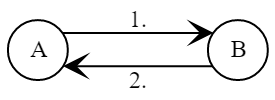
\includegraphics[width=0.5\textwidth]{pic/key_distribution-diffie-hellman}
    \caption{Обмен сообщениями в протоколе Диффи~---~Хеллмана\label{fig:key_distribution-diffie-hellman}}
\end{figure}

\begin{protocol}
    \item[(1)] Алиса выбирает случайное $2 \leq a \leq p - 1$
    \item[{}] $Alice \to \left\{ A = g ^ a \bmod p \right\} \to Bob$
    \item[(2)] Боб выбирает случайное $2 \leq b \leq p-1$
    \item[{}] Боб вычисляет сеансовый ключ $K = A ^ b \bmod p$
    \item[{}] $Bob \to \left\{ B = g ^ b \bmod p \right\} \to Alice$
    \item[(3)] Алиса вычисляет $K = B ^ a \bmod p$
\end{protocol}

Таким способом создан общий секретный сеансовый ключ $K$. За счёт случайного выбора значений $a$ и $b$ в каждом новом сеансе будет получен новой сеансовый ключ.

Протокол обеспечивает только генерацию новых сеансовых ключей (цель G10). В отсутствие третей доверенной стороны он не обеспечивает аутентификацию сторон (цель G1), а из-за отсутствия проходов с подтверждением владения ключом отсутствует аутентификация ключа (цель G8). Зато, так как протокол не использует длительные <<мастер>>-ключи, можно говорить о том, что он обладает свойством совершенной прямой секретности (цель G9).

Протокол можно использовать только с такими каналами связи, в которые не может вмешаться активный криптоаналитик. В противном случае протокол становится уязвим к простой атаке <<человек посередине>>\index{атака!<<человек посередине>>}.

\begin{figure}
    \centering
    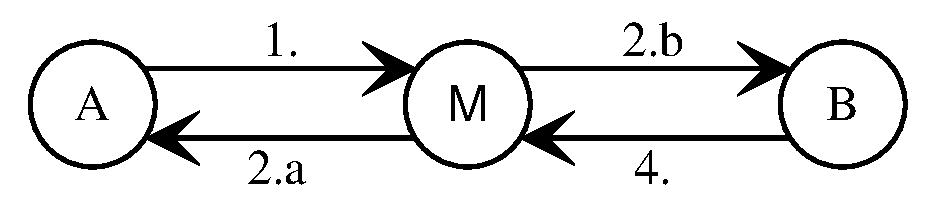
\includegraphics[width=0.67\textwidth]{pic/key_distribution-diffie-hellman-mitm}
    \caption{Схема взаимодействия участников в протоколе Диффи~---~Хеллмана при атаке <<человек посередине>>\label{fig:key_distribution-diffie-hellman-mitm}}
\end{figure}

\begin{protocol}
    \item[(1)] Алиса выбирает случайное $2 \leq a \leq p - 1$
    \item[{}] $Alice \to \left\{ A = g ^ a \bmod p \right\} \to Mellory~(Bob)$
    \item[(2)] Меллори выбирает случайное $2 \leq m \leq p-1$
    \item[{}] Меллори вычисляет сеансовый ключ для канала с Алисой
        \[K_{AM} = A ^ m \bmod p = g ^ {am} \bmod p\]
    \item[{}] $Mellory~(Alice) \to \left\{ M = g ^ m \bmod p \right\} \to Bob$
    \item[{}] $Mellory~(Bob) \to \left\{ M = g ^ m \bmod p \right\} \to Alice$
    \item[(3)] Алиса вычисляет сеансовый ключ для канала с Меллори (думая, что Меллори это Боб)
        \[K_{AM} = M ^ a \bmod p = g ^ { am } \bmod p\]
\pagebreak
    \item[(4)] Боб выбирает случайное $2 \leq b \leq p-1$
    \item[{}] Боб вычисляет сеансовый ключ для канала с Меллори (думая, что Меллори это Алиса)
        \[K_{BM} = M ^ b \bmod p = g ^ { bm } \bmod p\]
    \item[{}] $Bob \to \left\{ B = g ^ b \bmod p \right\} \to Mellory~(Alice)$
    \item[(5)] Меллори вычисляет сеансовый ключ для канала с Бобом
        \[K_{BM} = B ^ m \bmod p = g ^ { bm } \bmod p\]
\end{protocol}

В результате Алиса и Боб получили новые сеансовые ключи, но <<защищённый>> канал связи установили не с друг с другом, а со злоумышленником, который теперь имеет возможность ретранслировать или изменять все передаваемые сообщения между Алисой и Бобом.

Протокол Диффи~---~Хеллмана отличается от большей части протоколов распространения ключей из-за того, что не использует другие криптографические примитивы (функции шифрования, электронно-цифровой подписи или хеширования), но сам по себе является в некотором смысле криптографическим примитивом для построения более сложных протоколов. Он обеспечивает генерацию случайного числа в распределённой системе без доверенного центра. Причём ни одна из сторон не может заставить другую сторону использовать старый сессионный ключ, в отличие от, например, протокола Yahalom\index{протокол!Yahalom} из раздела~\ref{section-protocols-yahalom}.

Протокол можно изменить таким образом, чтобы вместо мультипликативной группы простого умножения использовать аддитивную группу сложения точек эллиптической кривой (см. раздел~\ref{section-math-ec-groups}). В этом случае стороны по прежнему будут выбирать некоторые случайные целые числа, но не возводить генератор-число в степень, а умножать генератор-точку на загаданное число.

\begin{protocol}
    \item[(0)] Стороны договорились о группе точек эллиптической кривой $\group{E}$, её циклической подгруппе $\group{G}$ мощности $n = \| \group{G} \|$ и генераторе $G$ группы $\group{G}$ (или хотя бы достаточно большой подгруппы группы $\group{G}$).
    \item[(1)] Алиса выбирает случайное $2 \leq a \leq n - 1$
    \item[{}] $Alice \to \left\{ A = a \times G \right\} \to Bob$
    \item[(2)] Боб выбирает случайное $2 \leq b \leq n - 1$
    \item[{}] Боб вычисляет точку $K = b \times A$
    \item[{}] $Bob \to \left\{ B = g \times G \right\} \to Alice$
    \item[(3)] Алиса вычисляет точку $K = a \times B$
\end{protocol}

В качестве нового сессионного ключа стороны могут выбрать, например, первую координату найденной точки $K$.

\index{протокол!Диффи~---~Хеллмана|)}\index{схема!Диффи~---~Хеллмана|)}

\subsection{Протокол Эль-Гамаля}\index{протокол!Эль-Гамаля|(}
\selectlanguage{russian}

\begin{figure}
    \centering
    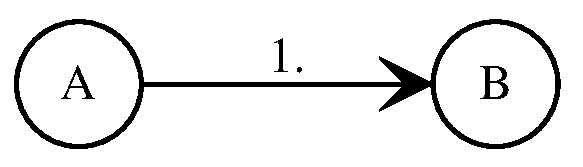
\includegraphics[width=0.5\textwidth]{pic/key_distribution-el-gamal}
    \caption{Взаимодействие участников в протоколе Эль-Гамаля\label{fig:key_distribution-el-gamal}}
\end{figure}

Протокол Эль-Гамаля (рис.~\ref{fig:key_distribution-el-gamal}, \cite{ElGamal:1984, ElGamal:1985}) за счёт предварительного распространения открытого ключа одной из сторон обеспечивает аутентификацию ключа для этой стороны. Можно гарантировать, что только владелец соответствующего закрытого ключа сможет вычислить сеансовый ключ. Однако подтверждение факта получение ключа (выполнение целей G1 и G8) не является частью протокола.

\begin{protocol}
    \item[(0)] Алиса и Боб выбирают общие параметры $p$ и $g$, где $p$ -- большое простое число, а $g$ -- примитивный элемент поля $\Z_p^*$.
    \item[{}] Боб создаёт пару из закрытого и открытого ключей $b$ и $K_B$:
        \[\begin{array}{l}
            b: 2 \leq b \leq p - 1, \\
            K_B = g^b \bmod p.
        \end{array}\]
    \item[{}] Открытый ключ $K_B$ находится в общем открытом доступе для всех сторон. Криптоаналитик не может подменить его -- подмена будет заметна.
    \item[(1)] Алиса выбирает секрет $x$ и вычисляет сеансовый ключ $K$
        \[ K = K_B^{x} = g^{bx} \bmod p. \]
        \[ Alice \to \left\{ g^x \bmod p \right\} \to Bob\]
    \item[(2)] Боб вычисляет сеансовый ключ
        \[ K = (g^x)^{b} = g^{bx} \bmod p. \]
\end{protocol}

Протокол не обеспечивает гарантию выбора нового сессионного ключа в каждом сеансе протокола (G10), а использование <<мастер>>-ключа $K_B$ для передачи сеансового ключа позволяет злоумышленнику вычислить все сессионные ключи из прошлых сеансов при компрометации закрытого ключа $b$ (цель G9).

\index{протокол!Эль-Гамаля|)}

\subsection{Взаимная аутентификация шифрованием}
\selectlanguage{russian}

К протоколам взаимной аутентификации принадлежит семейство протоколов, разработанных Ц.~Мацумото (\langen{Tsutomu Matsumoto}), И.~Такашима (\langen{Youichi Takashima}) и Х.~Имаи (\langen{Hideki Imai}) и названных по первым буквам фамилий авторов -- \emph{протоколы MTI}\index{протоколы!MTI}.

Здесь к открытым данным относятся:
    \[ p, ~~ g, ~~ \PK_A = g^a \mod p, ~~ \PK_B = g^b \mod p. \]
Каждый из пользователей $A$ и $B$ обладает парой долговременных ключей для \emph{схемы шифрования с открытым ключом}: закрытым ключом расшифрования $\SK$ и открытым ключом шифрования $\PK$.
\[ \begin{array}{ll}
    A: & ~ \SK_A = a, ~~ \PK_A = g^a \mod p, \\
    B: & ~ \SK_B = b, ~~ \PK_B = g^b \mod p. \\
\end{array} \]

\textbf{Протокол MTI}:
\begin{enumerate}
    \item Сторона $A$ генерирует случайное число $x, ~ 2\leq x\leq p-1$, создаёт и отправляет $B$ сообщение:
        \[ A \to B: ~ g^x \mod p. \]
    \item Сторона $B$ генерирует случайное число $y, ~ 2\leq y\leq p-1$, создаёт и отправляет $A$ сообщение:
        \[ A \leftarrow B: ~ g^y \mod p. \]
    \item Сторона $A$, используя открытые данные и полученное сообщение, создаёт сеансовый ключ:
        \[ K_A = (g^b)^x \cdot (g^y)^a = g^{bx+ay} \mod p. \]
    \item Сторона $B$, используя открытые данные и полученное сообщение, создаёт сеансовый ключ:
        \[ K_B = (g^x)^b \cdot (g^a)^y = g^{bx+ay} \mod p. \]
        Сеансовые ключи обеих сторон совпадают:
        \[ K_{A} =K_{B} = K. \]
\end{enumerate}

В описанном протоколе, как и в протоколе Эль-Гамаля\index{криптосистема!Эль-Гамаля}, происходит взаимная аутентификация сторон: открытые ключи сторон незаметно подменить невозможно. Наблюдая сообщения протокола, вычислить $g^{bx+ay}$ можно, только если известны значения $a,x$ или $b,y$, что представляет собой задачу дискретного логарифмирования, вычислительно трудную на сегодняшний день.


\subsection{Протокол Station-to-Station}\label{section-protocols-sts}\index{протокол!Station-to-Station|(}
\selectlanguage{russian}

Протокол STS (\langen{Station-to-Station},~\cite{Diffie:Oorschot:Wiener:1992})\index{протокол!Station-to-Station} предназначен для систем мобильной связи. Он использует идеи протокола Диффи~---~Хеллмана\index{протокол!Диффи~---~Хеллмана} и криптосистемы RSA\index{криптосистема!RSA}. Особенностью протокола является использование механизма электронной подписи\index{электронная подпись} для взаимной аутентификации сторон\index{аутентификация!взаимная}.

Предварительно стороны договорились об общих параметрах системы $p$ и $g$, где $p$ -- большое простое число, а $g$ -- примитивный элемент поля $\Z_p^*$.

Каждая из сторон $A$ и $B$ обладает долговременной парой ключей: закрытым ключом для расшифрования и создания электронной подписи $K_{\text{public}}$ и открытым ключом для шифрования и проверки подписи $K_{\text{public}}$.

\[\begin{array}{ll}
    A: K_{A,\text{private}}, K_{A,\text{public}}: \forall M : & \text{Verify}_A ( M, S_A( M ) ) = true, \\
                                                & D_A ( E_A( M ) ) = M, \\
    B: K_{B,\text{private}}, K_{B,\text{public}}: \forall M : & \text{Verify}_B ( M, S_B( M ) ) = true, \\
                                                & D_B ( E_B( M ) ) = M. \\
\end{array}\]

Где $\text{Verify}_A(\dots)$ это функция проверки электронной подписи на открытом ключе $K_{A, \text{public}}$, а $D_A$ -- функция расшифрования с использованием закрытого ключа $K_{A, \text{private}}$.

Протокол состоит из четырёх проходов, три из которых включают передачу сообщений (рис.~\ref{fig:key_distribution-sts}, \cite{Cheremushkin:2009}).

\begin{figure}
    \centering
    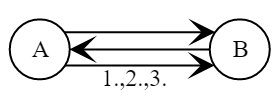
\includegraphics[width=0.5\textwidth]{pic/key_distribution-sts}
    \caption{Взаимодействие участников в протоколе STS\label{fig:key_distribution-sts}}
\end{figure}

\begin{protocol}
    \item[(1)] Алиса выбирает случайное число $R_A: 2 \leq R_A \leq p-1$.
    \item[{}] $Alice \to \left\{ A, m_A = g^{R_A} \bmod p \right\} \to Bob$

    \item[(2)] Боб выбирает случайное число $R_B: 2 \leq R_B \leq p-1$.
    \item[{}] Боб вычисляет сессионный ключ $K = m_A^{R_B} \bmod p$.
    \item[{}] $Bob \to \left\{ B, A, m_B = g^{R_B} \bmod p, E_K( S_B ( m_A, m_B )) \right\} \to Alice$

    \item[(3)] Алиса вычисляет сессионный ключ $K = m_B^{R_A} \bmod p$.
    \item[{}] Алиса проверяет подпись в сообщении $E_K( S_B ( m_A, m_B ))$.
    \item[{}] $Alice \to \left\{ A, B, E_K( S_A ( m_A, m_B ) ) \right\} \to Bob$

    \item[(4)] Боб проверяет подпись в сообщении $E_K( S_A ( m_A, m_B ))$.
\end{protocol}

Протокол обеспечивает арантию формирования новых ключей (G10), но не совершенную прямую секретность (G9).

Как показала атака Лоу 1996 года (\cite{Lowe:1996}, рис.~\ref{fig:key_distribution-sts-attack}), протокол не может гарантировать аутентификацию субъектов (цель G1), ключей (G7) и подтверждение владения сессионным ключом (G8). Хотя злоумышленник не может получить доступ к новому сессионному ключу, если протокол использовать только для аутентификации субъектов, Алиса может принять злоумышленника за Боба.

\begin{figure}
    \centering
    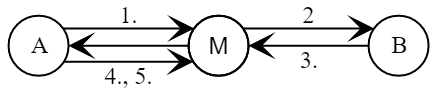
\includegraphics[width=0.67\textwidth]{pic/key_distribution-sts-attack}
    \caption{Схема взаимодействия участников в протоколе STS при атаке Лоу\label{fig:key_distribution-sts-attack}}
\end{figure}

\begin{protocol}
    \item[(1)] Алиса выбирает случайное число $R_A: 2 \leq R_A \leq p-1$.
    \item[{}] $Alice \to \left\{ A, m_A = g^{R_A} \bmod p \right\} \to Mellory~(Bob)$

    \item[(2)] $Mellory \to \left\{ M, m_A \right\} \to Bob$

    \item[(3)] Боб выбирает случайное число $R_B: 2 \leq R_B \leq p-1$.
    \item[{}] Боб вычисляет сессионный ключ $K = m_A^{R_B} \bmod p$.
    \item[{}] $Bob \to \left\{ B, M, m_B, E_K( S_B ( m_A, m_B )) \right\} \to Mellory$

    \item[(4)] $Mellory~(Bob) \to \left\{ B, A, E_K( S_B ( m_A, m_B )) \right\} \to Alice$

    \item[(5)] Алиса вычисляет сессионный ключ $K = m_B^{R_A} \bmod p$.
    \item[{}] Алиса проверяет подпись в сообщении $E_K( S_B ( m_A, m_B ))$.
    \item[{}] $Alice \to \left\{ A, B, E_K( S_A ( m_A, m_B ) ) \right\} \to Mellory~(Bob)$
\end{protocol}

После успешного завершения протокола Алиса уверена, что общается с Бобом.

Как и все остальные <<криптосистемы-протоколы>>, протокол Station-to-Station основывается на некотором внешнем источнике информации об открытых ключах участников, не подвергая сомнению корректность и надёжность этого источника. Что, в общем случае, неверно. Если информация о ключах участников нужно получать извне при каждом сеансе протокола (например, если участников много, и запомнить ключи всех возможности нет), то канал получения открытых ключей будет основной целью активного криптоаналитика для рассмотренных протоколов. Как от этого защититься с использованием примитивов асимметричной криптографии -- в разделе~\ref{section-protocols-asymmetric}.

\index{протокол!Station-to-Station|)}
